\section{Materials and methods}
%
We will first describe how a cross-validation procedure can be used to set peak-to-peak rejection thresholds globally (\textit{i.e.} same threshold for all sensors). This is what we call \textit{autoreject (global)}.

\subsection{Autoreject (global)}
\label{sec:auto_global}
We denote the data matrix by $X \in \real^{N \times P}$ with $N$ trials and $P$ features. These $P$ features are the $Q$ sensor-level time series, each of length $T$ concatenated along the second dimension of the data matrix, such that $P=QT$. We divide the data into $K$ folds (along the first dimension) with training set indices $\mathcal{T}_{k}$ and validation set indices $\mathcal{V}_{k}=[1..N] \setminus {\mathcal{T}_k}$ for each fold $k$ $(1 \leq k \leq K)$. For simplicity of notation, we first define the peak-to-peak amplitude for the $i$th trial and $j$th sensor as the difference between the maximum and the minimum value in that time series:
\begin{equation}
\mathcal{A}_{ij} = \max_{(j-1)T+1 \leq t \leq jT} (X_{it}) - \min_{(j-1)T+1 \leq t \leq jT} (X_{it}) \enspace .
\end{equation}
The set of indices of good trials $\mathcal{G}_k$ in which the peak-to-peak amplitude $\mathcal{A}_{ij}$ for any sensor does not exceed the candidate threshold $\tau$ are generated as
\begin{equation}
\mathcal{G}_k = \{i \in \mathcal{T}_{k} \suchthat \max_{1 \leq j \leq Q} \mathcal{A}_{ij} \leq \tau\}.
\end{equation}
By comparing the peak-to-peak threshold with the maximum of the peak-to-peak amplitudes, we ensure that none of the sensors exceed the given threshold. Once we have applied the threshold on the training set, it is necessary to evaluate how the threshold performs by looking at new data. For this purpose, we consider the validation set. We propose to compare the mean $\overbar{X_{\mathcal{G}_k}}(\tau)$ of good trials in the training set against the median $\widetilde{X_{\mathcal{V}_k}}$ of all trials in the validation set. Using root mean squared error (RMSE) the mismatch $e_{k}(\tau)$ reads as:
\begin{equation}
 e_{k}(\tau) = \fro{\overbar{X_{\mathcal{G}_k}}(\tau) - \widetilde{X_{\mathcal{V}_k}}}.
\label{eq:err} 
\end{equation}
Here, $\fro{\cdot}$ is the Frobenius norm. The rationale for using the median in the validation set is that it is robust to outliers. Indeed, it is far less affected by high-amplitude artifacts than the mean. The threshold with the best data quality (lowest mismatch $e_{k}(\tau)$) on average across the $K$ folds is selected as the optimal threshold. In practice $\tau$ is taken in a bounded interval $[\tau_{\min}, \tau_{\max}]$:
%
\begin{equation}
\tau_{\star} = \underset{\tau \in [\tau_{\min}, \tau_{\max}]} \argmin \frac{1}{K} \sum_{k=1}^{K}  e_{k}(\tau)
\label{eq:best_th}
\end{equation}
Note, that $\widetilde{X_{\mathcal{V}_k}}$ does not depend on $\tau$. Indeed, it would not be wise to restrict the validation set to good trials according to the value of $\tau$. As $\tau$ varies, it would lead to a variable number of validation trials, which would affect the comparison of RMSE across threshold values. The idea of using the median in the context of cross-validation has been previously proposed in the statistics literature in order to deal also with outliers~\citep{zheng1998cross, leung2005cross,de2003robust}.

Figure~\ref{fig:cross_val} (on page~\pageref{fig:cross_val}) shows how the average RMSE changes as the threshold varies for the MNE sample dataset~\citep{gramfort2013meg,mne}. At low thresholds, our model underfits as it drops most of the trials in the data resulting in a noisy average. On the other hand, at high thresholds, the model overfits retaining all the trials in the data including the high-amplitude artifacts. Here the candidate values of $\tau$ were taken on a grid. More details on how to solve \eqref{eq:best_th} will be given in Section~\ref{sec:bayesian_opt}.

\subsection{Autoreject (local)}
\label{sec:auto_local}

\begin{figure}[t]
	\centering
	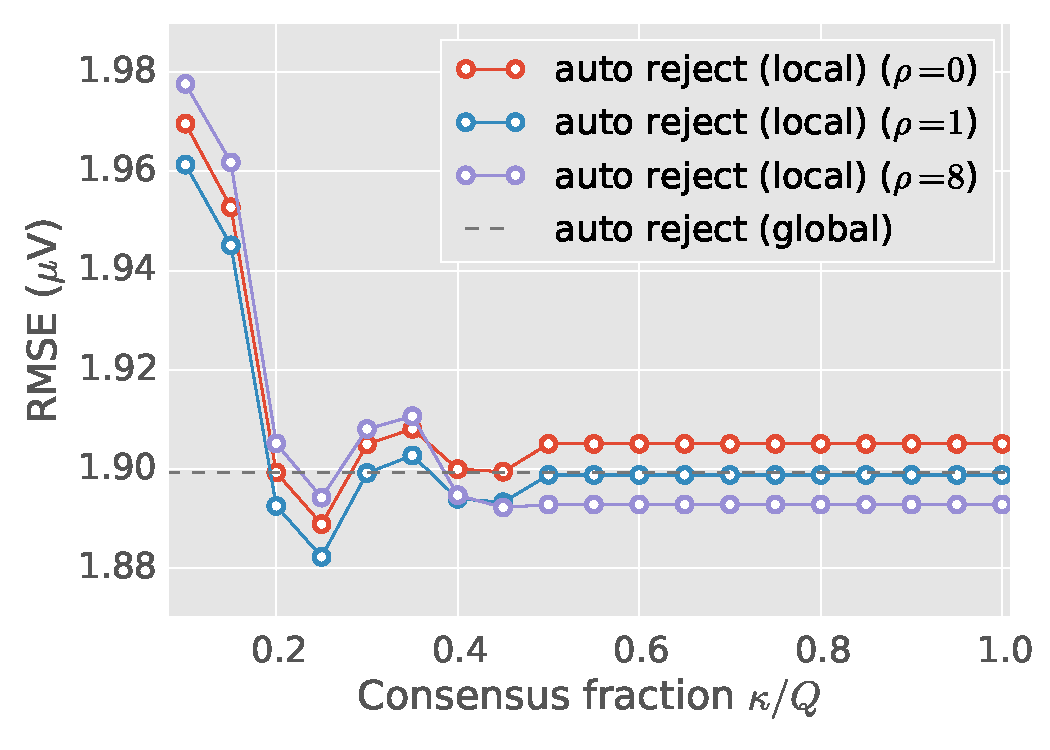
\includegraphics[width=0.65\linewidth]{figures/figure3.pdf}
    \caption[A schematic diagram explaining how \emph{autoreject (local)} works.]{A schematic diagram explaining how \emph{autoreject (local)} works. (A) Each cell here is an element of the transposed indicator matrix $C_{ij}^\top$ described in Section~\ref{sec:auto_local}. Sensor-level thresholds are found and bad segments are marked for each sensor. Bad segments shown in red are where $C_{ij}^\top=1$ (B) Trials are rejected if the number of bad sensors is greater than $\kappa$ and otherwise, the worst $\rho$ sensors (see Equation~\ref{eq:score}) are interpolated.}
    \label{fig:schematic}
\end{figure}

A global threshold common to all sensors, however, suffers from limitations. A common case of failure is when a single sensor is affected (locally or globally) by high-amplitude artifacts. In this case, $\max_{j} \mathcal{A}_{ij}$, which would be the peak-to-peak amplitude that is compared to the threshold, comes from this bad sensor. If the sensor is not repaired or removed, we might end up rejecting a large fraction of otherwise good trials, just because of a single bad sensor. This is certainly not optimal. In fact, a possibly better solution is to replace the corrupted signal in the sensor by the interpolation of the signals in the nearby sensors. A second observation is that sensors can have very different ranges of amplitudes depending on their location on the scalp. A threshold tuned for one sensor may not work as effectively for another sensor. Both of these observations are motivations for estimating rejection thresholds for each sensor separately.

Once we define sensor-wise rejection thresholds $\tau_{\star}^{j}$, we can define an indicator matrix $C_{ij} \in \{0, 1\}^{N \times Q}$ which designates the bad trials at the level of individual sensors. In other words, we have:
\begin{equation}
C_{ij} = \begin{cases} 
0, & \text{if } \mathcal{A}_{ij} \leq \tau^{j}_{\star} \\
1, & \text{if } \mathcal{A}_{ij} > \tau^{j}_{\star}
\end{cases}
\end{equation}
The schematic in Figure~\ref{fig:schematic}A shows a cartoon figure for this indicator matrix $C_{ij}$. Now that we have identified bad sensors for each trial, one might be tempted to interpolate all the bad sensors in each trial. However, it is not as straightforward since in some trials, a majority of the sensors may be bad. These trials cannot be repaired by interpolation and must be rejected. In some other cases, the number of bad sensors may not be large enough to justify rejecting the trial. However, it might already be too much to interpolate all the sensors reliably. In these cases, a natural idea is to pick the worst few sensors and interpolate them. This suggests an algorithm as described in Figure~\ref{fig:schematic}B. Reject a trial only if most sensors ``agree'' that the trial is bad, otherwise interpolate as many sensors as possible. We will denote by $\kappa$ the maximum number of bad sensors in a non-rejected trial and by $\rho$ the maximum number of sensors that can be interpolated. Note that $\rho$ is necessarily less than $\kappa$. The interpolation scheme for EEG uses spherical splines~\citep{perrin1989spherical} while for MEG it uses a Minimum Norm Estimates formulation with spherical harmonics~\citep{hamalainen1994interpreting}. The implementation is provided by MNE-Python~\citep{gramfort2013meg}.

The set of good trials $\mathcal{G}^{\kappa}_k$ in the training set $\mathcal{T}_k$ can therefore be written mathematically as:
%
\begin{equation}
\mathcal{G}^{\kappa}_{k} = \{i \in \mathcal{T}_k \suchthat \sum_{j=1}^{Q} C_{ij} < \kappa \} \enspace .
\end{equation}
%
In the remaining trials, if $\rho < \kappa$, one needs to define what are the worse $\rho$ sensors that shall be interpolated. To do this we propose to rank the sensors for ``badness'' according to a score. A natural strategy to set the score is to use the peak-to-peak amplitude itself:
%
\begin{equation}
s_{ij} = \begin{cases}
\mathcal{A}_{ij} & \text{if } C_{ij} = 1 \\
-\infty & \text{if } C_{ij} = 0
\end{cases}
\label{eq:score}
\end{equation}

The higher the score $s_{ij}$, the worse the sensor. The $-\infty$ score is for ignoring the good sensors in the subsequent step. The following strategy is used for interpolation.
%
%
If the number of bad sensors $\sum_{j'=1}^{Q} C_{ij'}$ is less than $\rho$ we will interpolate all of them. Otherwise, we will interpolate the $\rho$ sensors with the highest scores.
In other words, we interpolate at most $\mathrm{min}(\rho, \sum_{j'=1}^{Q} C_{ij'})$ sensors.
%
%
%
%
%
%
%
%
%
%
%

Denoting by $X^{\rho}_{\mathcal{G}^{\kappa}_k}$ the data in the training set after rejection and cleaning by interpolation, the RMSE averaged over $K$ folds for the parameter pair $(\rho, \kappa)$ therefore becomes:
%
\begin{equation}
\overbar{e}(\rho, \kappa) = \frac{1}{K} \sum_{k=1}^{K} \fro{\overbar{X^{\rho}_{\mathcal{G}^{\kappa}_k}} - \widetilde{X_{\mathcal{V}_k}}}
\end{equation}
where $\fro{\cdot}$ is the Frobenius norm.
Finally, the best parameters $\rho_{*}$ and $\kappa_{*}$ are estimated using grid search~\citep{hsu2003practical}.
%

\subsubsection{Data augmentation}
\label{sec:data_augmentation}

\begin{figure}[ht!]
    \centering
    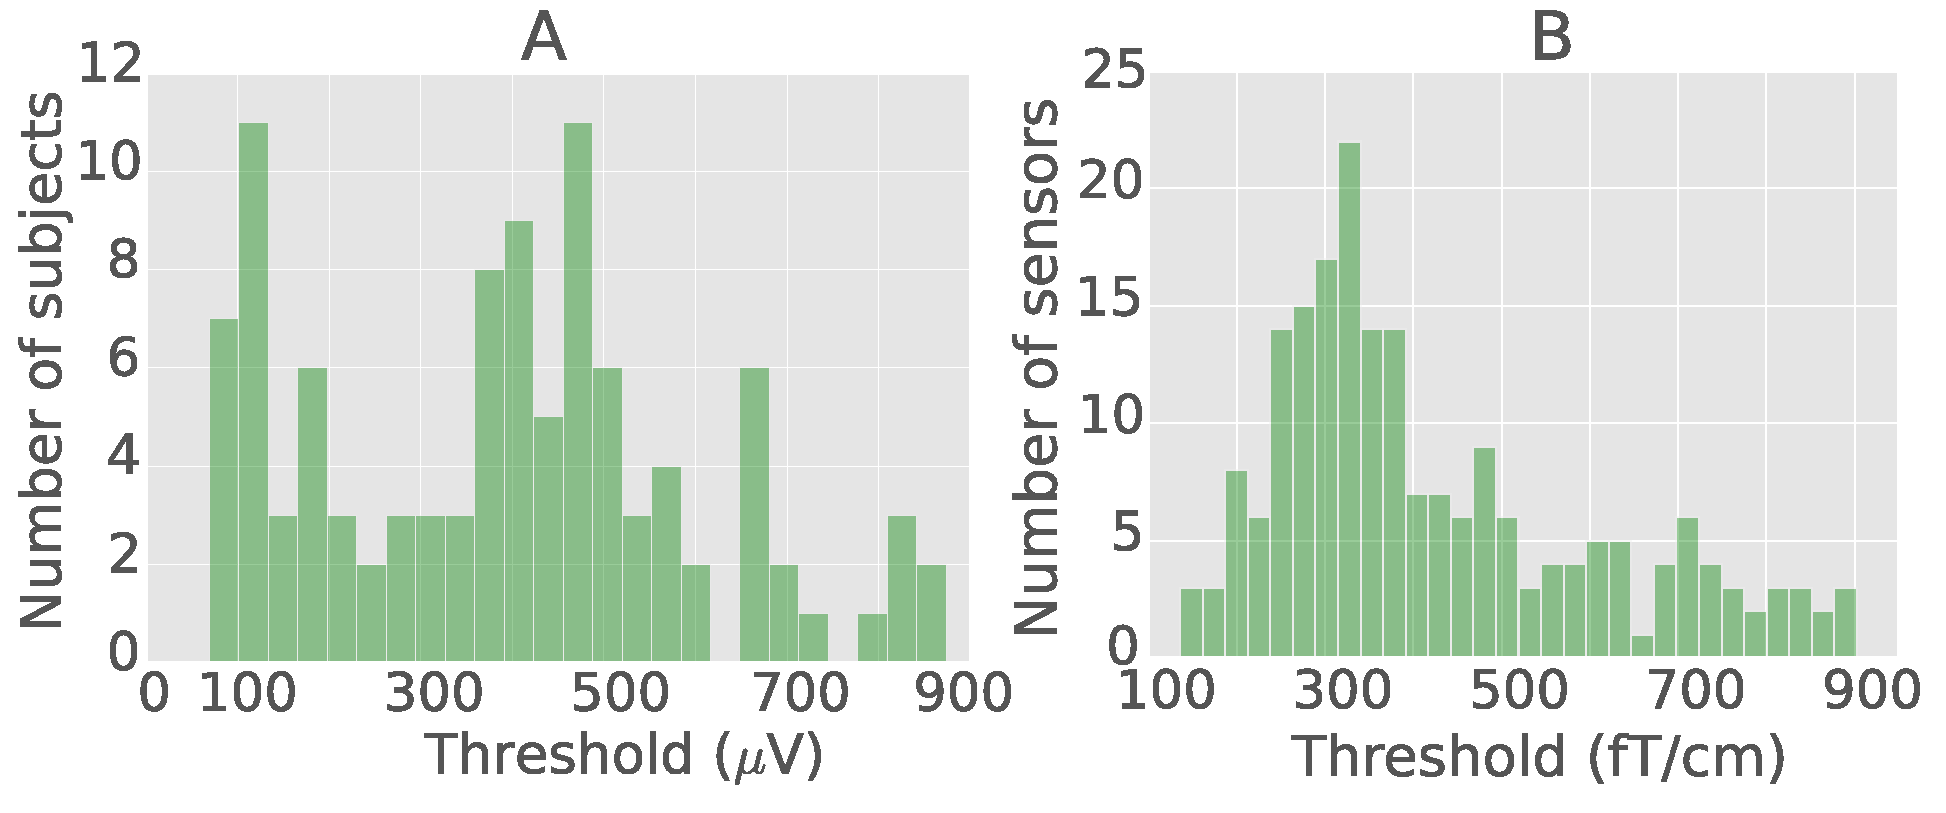
\includegraphics[width=0.8\linewidth]{figures/figure2.pdf}
    \caption[Sequential Bayesian optimization cross-validation curves]{(A) and (B) The cross-validation curve obtained with sequential Bayesian optimization (see Section~\ref{sec:bayesian_opt} for an explanation) for a regular (MEG 2523) and a globally bad sensor (MEG 2443) from the MNE sample dataset. The mean \ac{RMSE} is shown in red circles with the standard deviation in red shades. Vertical dashed line marks the estimated threshold. (C) and (D) Histogram of peak-to-peak amplitudes of trials in the sensor. The histograms are computed separately for the real data (red) and the data interpolated from other sensors (blue). The estimated optimal threshold correctly marks all the trials as bad for the globally bad sensor.}
    \label{fig:cross_val_hist}
\end{figure}

In practice, cross-validation does not work for a globally bad sensor since all the trials are corrupted. In this scenario, the optimal threshold for this bad sensor should be lower than the lowest peak-to-peak amplitude so that all the trials for that sensor are marked as bad. However, even the median of the validation set has been corrupted. The algorithm therefore attempts to keep as many trials as necessary for the average to be close to the corrupted median. Thus, the estimated threshold ends up being higher than what would have been optimal. Recall from Figure~\ref{fig:cross_val} that this is the classic case of an overfitting model. A common strategy in machine learning to reduce overfitting is data augmentation~\citep{krizhevsky2012imagenet}. It basically boils down to using the properties of the data (in our case, this being the physics of the system) to generate additional plausible data.

To implement data augmentation in our model, we interpolate each sensor from all the other $Q-1$ sensors and by doing so, we double the number of trials in the data. In the augmented data, half of the trials contain sensor data. The augmented data matrix is $X^{\textrm{aug}} \in \real^{2N \times P}$. With the augmented data, the median is now closer to the uncorrupted median of the data in that sensor. During cross-validation the folds were stratified so that the number of interpolated trials and original trials in each fold were roughly equal.

\subsection{Search for optimal thresholds using Bayesian optimization}
\label{sec:bayesian_opt}
Now that we have formalized the problem and our approach, we must estimate the threshold $\tau_{\star}$ which minimizes the error defined in Equation~\eqref{eq:err}. A na\"ive strategy is to define a set of equally spaced points over a range of thresholds $[\tau_{\min}, \tau_{\max}]$. The estimated threshold would be the one which obtains the lowest error among these candidate threshold. This is the approach taken in Figure~\ref{fig:cross_val}. The range of thresholds is easy to set as it can be determined from the minimum and maximum peak-to-peak amplitude for the sensor in the augmented data matrix $X^{\textrm{aug}}$. However, it is not obvious how to set the spacing between the candidate thresholds, and experiments showed that varying this spacing could impact the results. If the candidate thresholds are far apart, one might end up missing the optimal threshold. On the other hand, if the thresholds are very dense, it is computationally more demanding.

This motivated us to use Bayesian optimization~\citep{snoek2012practical, bergstra2011algorithms} to estimate the optimal thresholds. It is a sequential approach which decides the next candidate threshold to try based on all the observed thresholds so far. It is based on maximizing an acquisition function given an objective function of samples seen so far (data likelihood) and the prior (typically a \ac{GP}~\citep{rasmussen2006gaussian}). The objective function in our case is the mean cross-validation error as defined in Equations~\eqref{eq:err}. To obtain the next iterate, an acquisition function is maximized over the posterior distribution. Popular choices of the acquisition function include ``probability of improvement'', ``expected improvement'' and ``confidence bounds of the \ac{GP}''~\citep{snoek2012practical}. We pick ``expected improvement'' as it balances exploration (searching unknown regions) and exploitation (maximizing the improvement) strategies without the need of a tuning parameter. For our analysis, we use the scikit-optimize\footnote{https://scikit-optimize.github.io} implementation of Bayesian optimization, which internally uses the Gaussian process module from scikit-learn~\citep{scikit-learn}.

Figure~\ref{fig:cross_val_hist}A and \ref{fig:cross_val_hist}B show the cross-validation curve for a regular sensor and a globally bad sensor in the MNE sample dataset~\citep{mne,gramfort2013meg}. The RMSE is evaluated on thresholds as determined by the Bayesian optimization rather than a uniform grid. These plots also illustrate the arguments presented in Section~\ref{sec:data_augmentation} with respect to data augmentation. The histograms in Figure~\ref{fig:cross_val_hist}C for the interpolated data and the real data are overlapping for the regular sensor. Thus, the estimated threshold for that sensor marks a trial as outlier if its peak-to-peak values is much higher than the rest of the trials. However, in the case of a globally bad sensor, the histogram (Figure~\ref{fig:cross_val_hist}D) is bimodal -- one mode for the interpolated data and one mode for the real data. Now, the estimated threshold is no longer marking outliers in the traditional sense. Instead, all the trials belonging to that sensor must be marked as bad.
